% 
%    

%   . You can include graphics by using the command \includegraphics[scale=A fraction you pick]{FILENAME.png}  #this could be a screenshot
\documentclass[11pt]{article}
\usepackage{fancyhdr}
\usepackage[english]{babel}

\usepackage{amssymb}

\usepackage{graphicx,color,url,hyperref}

\setlength{\parindent}{0pt}
\setlength{\parskip}{5pt plus 1pt}
\setlength{\headheight}{13.6pt}

\newcommand{\R}{\mathbb{R}}

\usepackage{graphicx,color,url,hyperref}
\usepackage{epsfig}
\setlength{\parindent}{0pt}
\setlength{\parskip}{5pt plus 1pt}
\setlength{\headheight}{13.6pt}

\usepackage[margin=1in]{geometry}

\newcommand\question[2]{\vspace{.25in}\hrule\textbf{#1: #2}\vspace{.5em}\hrule\vspace{.10in}}

\pagestyle{fancyplain}

\chead{\textbf{Math 1550 HW1 Solution}}
\rhead{Math 1550, 09.14.20}
\lhead{Sunny Lee}

\begin{document}\raggedright

\subsubsection*{a.  1.1, \#1c} 
\vskip1em %Skips vertical space and you can increase or decrease the "em" space for example \vskip2em skips twice as far; you can also hit return twice to go to the next line.
\emph{Solution.} $\{4, 56, 6608, 87370976, 1.5267375419\times 10^{16}\}$  % we use $ $ for inline mathematical text and we need the backslash for getting the curly brackets to appear
\vskip1em

\subsubsection*{b. 1.1, \#1d} 
\vskip1em
\emph{Solution.} $\{1, 1, 1, 1, 1\}$
\vskip1em

\subsubsection*{c. 1.1, \#2a} 
\vskip1em
\emph{Solution.} $a_{n+1} = 3, a_{0} = 3$
\vskip1em

\subsubsection*{d. 1.1, \#2d} 
\vskip1em
\emph{Solution.} $a_{n+1} = 2^n + a_{n}, a_{0} = 1$
\vskip1em

\subsubsection*{e. 1.1, \#3c} 
\vskip1em
\emph{Solution.} $a_{n+1} = a_{n} + a_{n-1} + \cdots + a_{0} + n, a_{0} = 1$
\vskip1em

\subsubsection*{f. 1.1, \#3d} 
\vskip1em
\emph{Solution.} $a_{n+1} = 7(3^n) + a_{n}, a_{0} = 1$
\vskip1em

\subsubsection*{g. 1.1, \#4a} 
\vskip1em
\emph{Solution.} $\{1, \frac{1}{2}, \frac{1}{4}, \frac{1}{8}, \frac{1}{16}\}$
\vskip1em

\subsubsection*{h. 1.1, \#5c} 
\vskip1em
\emph{Solution.} $\{4, 56, 6608, 87370976\}$
\vskip1em

\pagebreak
\subsubsection*{i. 1.2, \#1} 
\vskip1em
\emph{Solution.} 
\vskip1em 

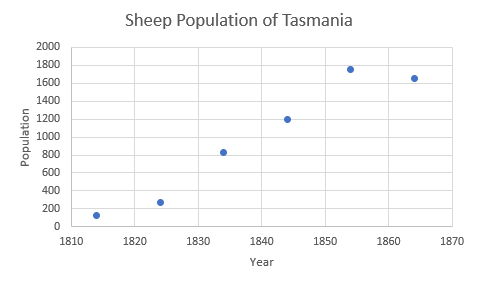
\includegraphics{population.png}
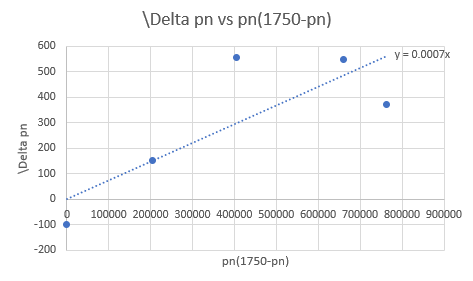
\includegraphics{delta.png}
\vskip1em
By using the difference equation for logistic regression $\Delta p_{n+1} = kp_{n}(M - p_{n})$,
and the Sheep population of Tasmania, we can assume the carrying capacity is 1750. 
So, using 1750 as our carrying capacity, we can plot the $\Delta p_{n}$ vs $pn*(1750-pn)$ 
on a graph. With this graph, we can also fit a linear regression line to find 
our value of k to model our difference equation: 
\begin{center}
    $\Delta p_{n+1} = .0007p_{n}(1750 - p_{n}) $
\end{center}
\vskip1em

\end{document}
